\subsection{Methodologies and Experiments}
In this section, we design experimental methodology to rigorously explore the range of possible approaches to dealing with barren plateaus in QNN/VQA development, thus leading to answering the study research question (see Section \ref{Problem Section}).

\subsubsection{Research Context}

\almarginpar{I cannot fit it below, so I include it here: Are the Table 1 elements in any way related to the experimental work? How? Is the number of experiments determined by the cases included in the table? Any relation with Figure 9?}
As explained in the previous section (Section \ref{Literature Review section}), the VQA approach to circuit design for QNN construction overcomes many constraints of the NISQ devices. It allows the construction of trainable circuits, which support development of practical applications in optimisation and machine learning.
However, we have observed the existence of barren plateaus, causing the variance of the cost function gradient to vanish exponentially with the number of qubits.
We have thus investigated three methods to mitigate this phenomenon, i.e. by using a local cost function with shallow circuits, by relying on the identity block and by utilising layerwise learning \cite{cerezoCostFunctionDependent2021, liuParameterInitializationMethod2021, skolikLayerwiseLearningQuantum2021}.

In the following sections, we will answer the study research question (see Section \ref{Problem Section}) by conducting a series of experiments, with different methods are applied to the same objects, this process is known as \emph{technology-oriented empirical research} \cite{wohlinExperimentationSoftwareEngineering2012}.

We summarise the adopted research process in Figure \ref{Research Activities Figure}.
Our main objects and the different technical treatments for the experiment are discussed in section \ref{Objects section}, the two phases of the experiment in section \ref{Research Activities section}, and finally the confirmation of results from the experiment in section \ref{Data Collecting Section}.
\almarginpar{You cannot just dump the figure with the research process, you need to explain what is in it, i.e. Figure 9 and the details of its three phases as related to sections 3.1.2 (where is it in the figure?), 3.1.3 (first and second phase), and what happened to the third? You still need to describe it}

\begin{figure}
    \centering
    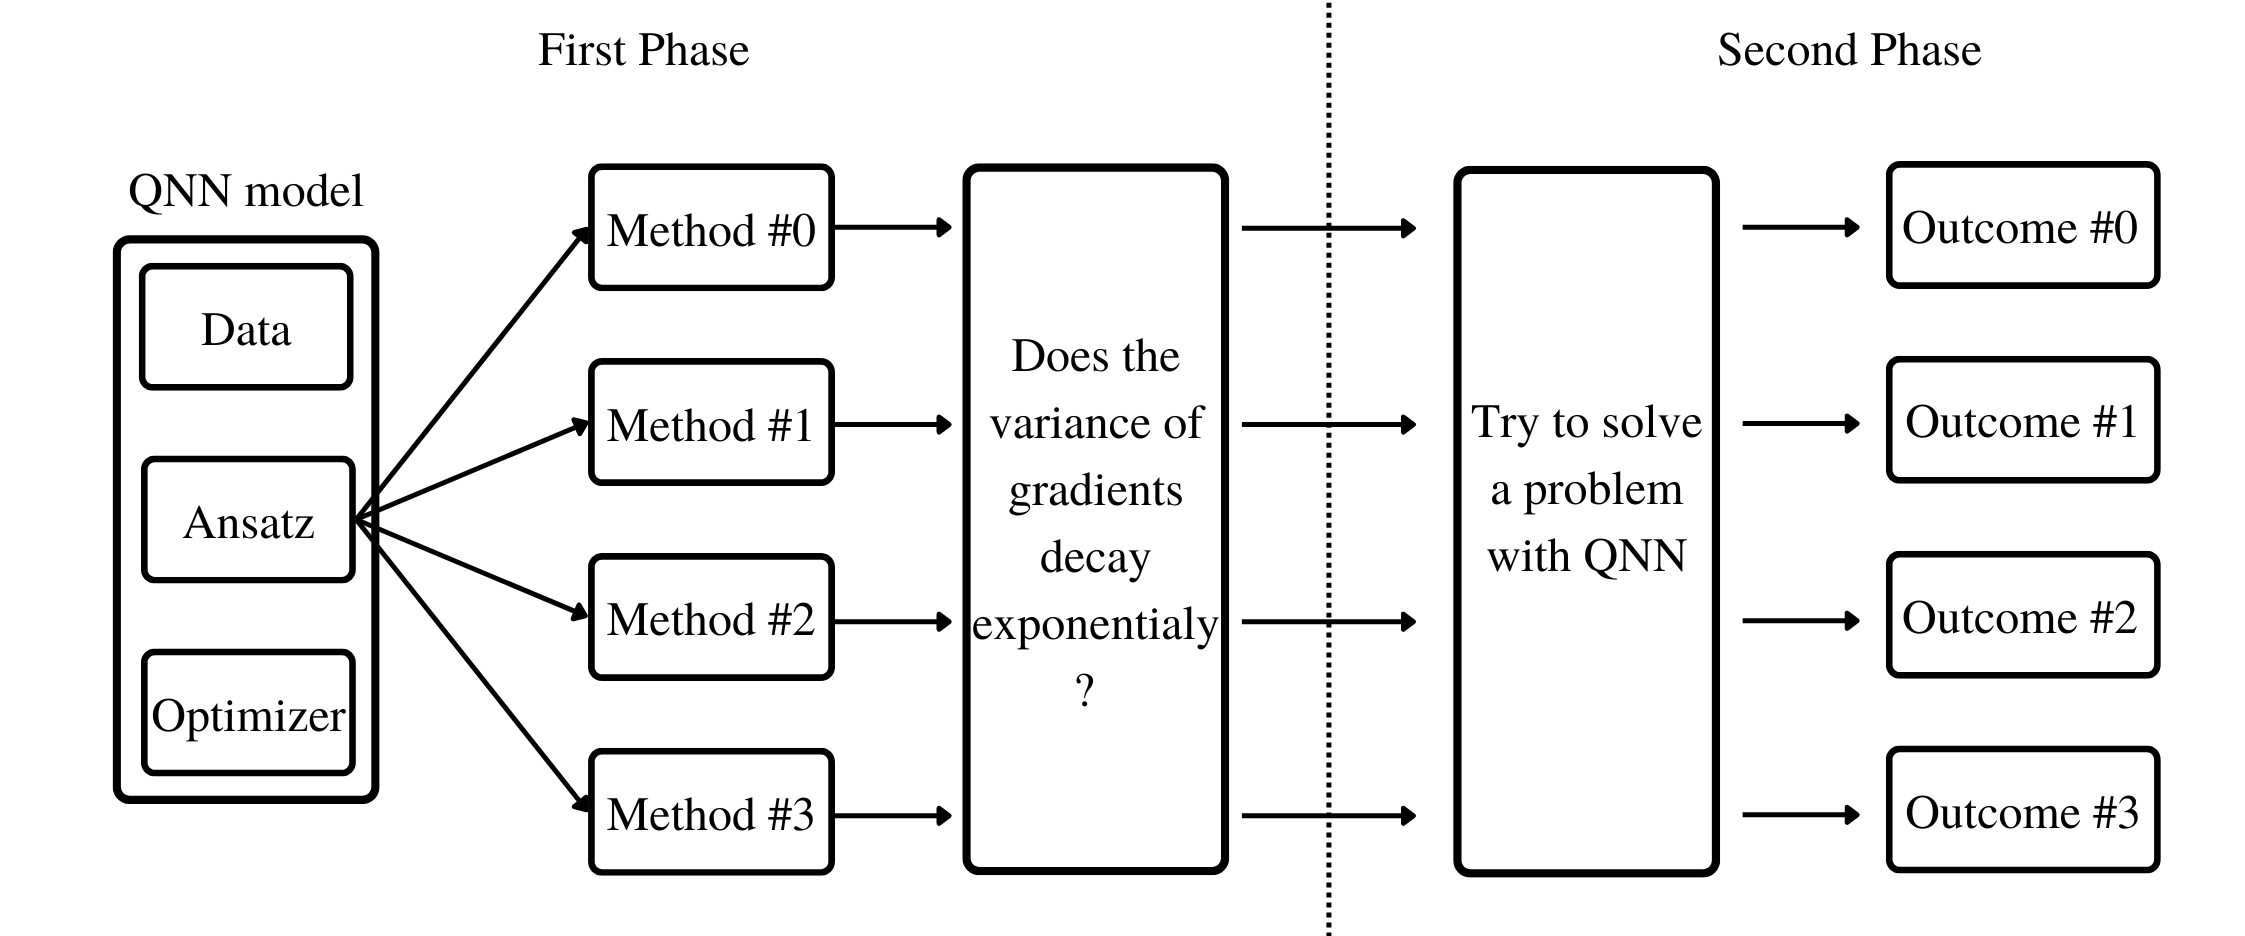
\includegraphics[width=\textwidth]{./ResearchDesign/Appendices/ExperimentDiagram.png}
    \caption{
        The adopted research process.
    }
    \label{Research Activities Figure}
\end{figure}

\subsubsection{Objects and Parameters}\label{Objects section}
According to the research design guidelines by Wohlin et al \cite{wohlinExperimentationSoftwareEngineering2012}, we will need to identify the experiment object and the parameters.
While the object is the main entity that is studied in the experiment, the parameters are the treatments applied to the object.
One advantage of the empirical experiment is that we can have total control of the experiment environment.
As per the literature review (see Section \ref{Literature Review section}), we have identified the object of study is the QNN model.
The parameters that we can apply to the object are:
\begin{itemize}
    \item \textbf{The ansatz choice.} Qiskit framework offers a wide range of ansatz, refer to the circuit library in Section \ref{Resources section};
    \item \textbf{The ansatz configuration.} The ansatz object from Qiskit is mutable, which means we can configure their properties to fit the experiment activities. For example, the number of qubits, repetition of layers, and initial parameters.
    \item \textbf{The cost function operator.} We can implement a measurement operation at the end of the parameterised quantum circuit to act as the output of the cost function. We discussed two styles of cost functions in Section \ref{Shallow Circuits, Local Cost Function section};
    \item \textbf{The method to mitigate barren plateaus.} We have reviewed three methods in Section \ref{Literature Review section}, and each of them configure or traine the ansatz differently (see Table \ref{quick comparison of methods}). Note that QCNN is out of scope of our experiment.
\end{itemize}

\subsubsection{Research Activities} \label{Research Activities section}
\textbf{In the first phase, we reproduce the barren plateaus phenomenon.}
We can use Qiskit \cite{Qiskit} to construct the ansatzes.
For the same ansatz, we implement four different methods (see Figure \ref{Research Activities Figure} and Table \ref{implementation of methods table}).
By definition of barren plateau as discussed in Section \ref{Literature Review section}, we would expect the shrinking rate of the variace values to be \textit{exponentially} (see Figure \ref{Variance Shrinking demo}) if the initial parameter has landed in a barren plateau.
We keep track of the variance and the number of qubits to see if the variance is shrinking at this rate.
The result of the first phase is the shringking rates of the same ansatz applied with different treatments.

\textbf{In the second phase, we implement the QNNs and measure their performances}.
With the ansatzes developed from the first step, we can implement the QNN models to test their performances.
The QNN models will be trained with standard data sets provided by Qiskit (refer to Section \ref{Resources section}).

The results of the research activities are discussed in the Subsection \ref{Data Collecting Section}.

\begin{table}[]
    \centering
    \begin{tabular}{|p{3cm}|p{2cm}|p{2cm}|p{2cm}|p{2cm}|}
        \hline
        \textbf{Method /\newline Aspect}      & \textbf{\#0:\newline No restrictions} & \textbf{\#1:\newline Local cost function, shallow circuits} & \textbf{\#2:\newline Identity Blocks} & \textbf{\#3:\newline Layerwise learning} \\
        \hline \hline
        \raggedright\emph{Ansatz depth}       & Any length                            & Bounded                                                     & Any length                            & Any length                               \\
        \hline
        \raggedright\emph{Cost Function}      & Global                                & Limited                                                     & All qubits                            & All qubits                               \\
        \hline
        \raggedright\emph{Initial Parameters} & Randomised                            & Randomised                                                  & Restricted                            & Restricted                               \\
        \hline
    \end{tabular}
    \caption{
        A comparison of different methods that applied to the ansatz in phase 1.
        The method $\#$0 is widely applied in construction of QNN ansatzes.
        The other three methods are discussed in Section \ref{Literature Review section}.
    }
    \label{implementation of methods table}
\end{table}


\begin{figure}
    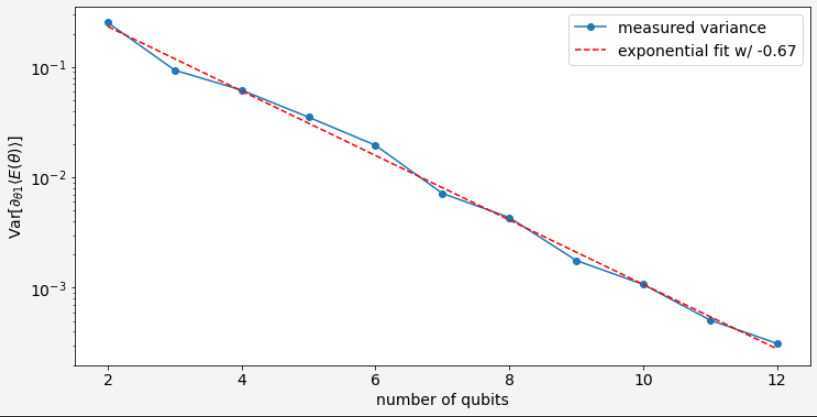
\includegraphics[width=\textwidth]{./ResearchDesign/Appendices/VarianceShrinking.png}
    \caption{
        An example of the barren plateaus phenomenon occurs in a QNN model.
        The variance of the gradient shrinks \textit{exponentially} with the number of qubits.
        Barren plateaus phenomenon prevents optimisation algorithms from navigating the cost function landscape efficiently.
    }
    \label{Variance Shrinking demo}
\end{figure}


\subsubsection{Criteria}
\label{Criteria section}
\almarginpar{I am not sure you provide all these details}We can compare the data with these criteria:
\begin{itemize}
    \item The quality of the solution;
    \item Loss values per iteration;
    \item The size of the circuit (circuit depth);
    \item The size of the qubit registry (circuit width);
    \item The time required to execute the circuit.
\end{itemize}

\subsubsection{Data Collecting Method}
\label{Data Collecting Section}
\almarginpar{You mention the "expertiments" for the first time? BTW, clearly these are a series of experiments not one experiment!}
Here we discuss our method to collect the data from the series of \emph{experiments}.

The output of the first phase is Qiskit ansatz objects that contain the number of qubits, the depth of the circuit (rep), and the parameter initialised randomly (refer to the Qiskit document for further detail - Section \ref{Resources section}).
Moreover, the ansatz object in Qiskit is mutable, which means we can modify the ansatzes properties in the second phase.

For the second phase, we need to record three different outputs of the three methods accordingly,
\almarginpar{Would this make 9 possible outcomes not 6? Why not 16 according to Table 1?}
with the criteria defined in Subsection \ref{Criteria section}.
The result is a table with the rows of criteria in the Subsection \ref{Criteria section} with each method as rows.
With this data, we can decide whether to reject the null hypothesis or not.

For the null hypothesis case, it means that the methods' performances are relatively the same, and we conclude the experiment.
We will have the result as a table for comparison, which satisfies hypothesis H1.
Then, we need to synthesise the table to answer the research question and verify hypothesis H2.
For example, the method $X$ is the best for the complexity.
\almarginpar{Note that H1 and H2 are not the hypotheses at all! You have clearly listed some objectives to achieve and you are not testing any hypotheses - the research methodology is very poor!}
Finally, we summarise the research results and present the findings.

\subsubsection{Resources} \label{Resources section}
Most of our required resources are open-sources:
\begin{itemize}
    \item Python 3.6+: \url{https://www.python.org/downloads/}
    \item Jupyter Notebook: \url{https://jupyter.org/}
    \item Qiskit: \url{https://qiskit.org/}
    \item IBM Quantum: \url{https://quantum-computing.ibm.com/}
    \item Qiskit circuit library: \url{https://qiskit.org/documentation/apidoc/circuit_library.html}
\end{itemize}

To prepare the quantum emulator on a local machine, we first install Python and Anaconda for programming language support and Jupyter Notebook as a code editing tool.
Then we follow the official instruction from Qiskit \cite{Qiskit} to install the necessary packages.
We can start working with Qiskit in a Jupyter Notebook file.

\almarginpar{Python "kernel"? do you mean "API" \\ - How about "python environment"? A notebook kernel is a “computational engine” that executes the code contained in a Notebook document.}The other option is to use the provided Python notbook environment provided by IBM Quantum with Qiskit pre-installed.
While this is a convenient choice for online presentation or remote working because of instant access, this server has shortcomings.
The maximum ram for open access is only 8 Gigabytes, and the processing power is limited.

The quantum emulator from Qiskit is capable of simulating up to 32 qubits.
On the other hand, the actual quantum hardware from IBM is limited to 5 qubits for open access.

\almarginpar{It also offers custom ansatz design, would you explore this option, why not?}Qiskit offers various pre-defined ansatz designs, namely \textit{EfficientSU2, PauliTwoDesign, RealAmplitudes, NLocal}, and \textit{TwoLocal}.
The Qiskit also allows custom parameterized circuits to be used as ansatzes.
However, we will use the ansatz \todo{insert ansatz name here} \textit{RealAmplitudes} to implement the QNN model in our experiment due to its popularity in quantum machine learning studies and implementation.
% They are popular and frequently studied in quantum chemistry, quantum machine learning, and especially the investigation of barren plateaus.
% However, \almarginpar{Not true!}\emph{they are based on the two ansatzes, NLocal and TwoLocal}.
% To construct the ansatz as discussed in Section \ref{Research Activities section}, we can use the NLocal and TwoLocal circuits provided.


\subsubsection{Success Condition}
The experiment will be concluded when these conditions are met:
\begin{itemize}
    \item We have QNN ansatzes that can produce barren plateaus;
    \item The three methods are implemented as Python scripts and ready for demonstration;
    \item The data from the three methods are evaluated against the criteria.
\end{itemize}